\documentclass[oneside]{VUMIFPSkursinis}
\usepackage{algorithmicx}
\usepackage{algorithm}
\usepackage{algpseudocode}
\usepackage{amsfonts}
\usepackage{float}
\usepackage{amsmath}
\usepackage{bm}
\usepackage{caption}
\usepackage{hyperref}
\usepackage{color}
\usepackage{float}
\usepackage{graphicx}
\usepackage{listings}
\usepackage{subfig}
\usepackage{ltablex}
\usepackage{longtable}
\usepackage{wrapfig}
\usepackage{enumitem}
\usepackage{subfig}
\usepackage{caption}
\usepackage{pbox}
\renewcommand{\labelenumii}{\theenumii}
\renewcommand{\theenumii}{\theenumi.\arabic{enumii}.}
\renewcommand{\labelenumiii}{\theenumiii}
\renewcommand{\theenumiii}{\theenumii\arabic{enumiii}.}
% Titulinio aprašas
\university{Vilniaus universitetas}
\faculty{Matematikos ir informatikos fakultetas}
\department{Programų sistemų katedra}
\papertype{Projektinis darbas}
\title{Internetinio banko tinklalapis}
\titleineng{Maketų analitiniai vertinimai}
\status{3 kurso 3 grupės studentai}
\author{Justas Tvarijonas}
\secondauthor{Džiugas Mažulis}   
\thirdauthor{Michal Stankevič}   
\supervisor{Kristina Lapin, Doc., Dr.}
\date{Vilnius – \the\year}

\begin{document}
\maketitle
\sectionnonum{Anotacija}
\subsectionnonum{Darbo tikslas}
Įvertinti 3-ių sukurtų maketų panaudojamumą ir pateikti išvadas, kaip toliau tęsti projektą. Šiam tikslui įgyvendinti išsikėlėme šiuos uždavinius:
\begin{enumerate}
	\item Kiekvienam maketui atlikti euristinį tikrinimą,
	\item Kiekvienam maketui atlikti pažintinę peržvalgą,
	\item Nustatyti tolimesnę projekto eigos kryptį.
\end{enumerate}
\subsectionnonum{Darbo pasiskirstymas}
\begin{itemize}
	\item Justas Tvarijonas - tvarijonasjustas@gmail.com
	\item Džiugas Mažulis - džiugas.mažulis@gmail.com
	\item Michal Stankevič - michal.stankevic@gmail.com 
\end{itemize}
\tableofcontents
\sectionnonum{Įvadas}
\subsectionnonum{Dalykinė sritis}
Internetinė bankininkystė.
\subsectionnonum{Probleminė sritis}
Vartotojo grafinės sąsajos išmokstamumo gerinimas, pagrindinėms funkcijoms pasiekti atliekamų žingsnių bei klaidų mažinimas.
\subsectionnonum{Naudotojai}
Banko klientas - turi galimybę atlikti mokėjimus, peržiūrėti sąskaitos išrašus, kurti mokėjimo ruošinius, ieškoti reikalingos informacijos.
\subsectionnonum{Darbo pagrindas}
Trečiojo laboratorinio darbo reikalavimai.
\section{Džiugo Mažulio maketo vertinimas}
\subsection{Euristinis tikrinimas}
% nesu tikras ar šitų skyrių prieš lentelę reikia
\subsubsection{Metodas}
Euristinis tikrinimas buvo atliktas remiantis dešimt Nielseno patobulintų euristikų sąrašu, bei jų išdėstymų 8 paskaitos skaidrėse.
\subsubsection{Teigiami įspūdžiai}
Justo Tvarijono vertinimas
\begin{itemize}
	\item Atlikus svarbesnius veiksmus vartotojas yra aiškiai informuojamas apie jų sėkmingą/nesėkmingą atlikimą (Būsenos matomumas).
	\item Meniu juosta yra pasiekiama viso sistemos naudojimosi metu, taip vartotojui suteikiama galimybė pereiti į kitus langus arba atsijungti neverčiant vartotojo pirma nuvykti į pradinį puslapį (Naudojimo lankstumas ir našumas).
	\item Tą pačią funkciją(šiuo atveju vietinius pavedimus) galima pasiekti skirtingais būdais reikalaujančiais skirtingo kiekio veiksmų, taip vartotujui suteikiant didesnę pasirinkimo laisvę (Navigacijos šuoliai).
	\item Beveik visi naudojami terminai yra naudotini realiame pasaulyje, taip vartotojui žymiai patogiau orientuotis sistemoje(Sistemos atitikimas realiam pasauliui).
	\item Vietinių mokėjimų lange galima rasti ne tik įvedimo laukus, bet ir mokėjimo ruošinių langą, taip išvengiant perteklinių langų naudojimo (Estetika ir minimalizmas).
	\item Radus klaidas atliekas svarbesnius veiksmus vartotojui aiškiai paaiškinimas, kur ir kodėl įvyko klaida (Klaidų atpažinimo rėmimas).
\end{itemize}
\subsubsection{Defektų sąrašas}
\begin{center}
\begin{longtable}[!htb]{|p{3.5cm}|p{3.5cm}|p{8.1cm}|}
	\caption{Justo Tvarijono vertinimas}
	\endfirsthead
	\endhead
  \hline
	Euristika & Defekto sunkumas & Komentaras \\ \hline
	Būsenos matomumas & Vidutinis & Vartotojas savo buvimo vietą mato tik būdamas pirmame hierarchijos sluoksnyje, jam einant į gylesnius sluoksnius, jis gali užmiršti kokioje vietoje yra. \\ \hline
	Sistemos atitikimas realiam pasauliui & Lengvas & Vietinių mokėjimų lange vartotojui gali būti ne akivaizdu, ką reiškia terminas "Gavėjo pavadinimas" \\ \hline
	Naudotojo valdomas dialogas & Vidutinis & Languose nėra grįžimo atgal mygtukų, vienintelis būdas grįžti yra naudojantis mygtukų juosta. \\ \hline
	Klaidų prevencija \label{lentele:klaiduPrevencijaJ} &\hyperref[fig:klaiduPrevencijaMygtukai]{Didelis} & Vietinių mokėjimų lange mygtukai "Patvirtinti mokėjimą" ir "Išsaugoti duomenis" nėra atskirti tarpais, bei paspaudus "Patvirtinti mokėjimą" nėra atliekamas papildomas paklausimas ar vartotojas nori atlikti tą mokėjimą, todėl yra galimybė, kad vartotojas norėdamas išsaugoti duomenis prieš savo valią atliks mokėjimo pavedimą\\ \hline
	Klaidų prevencija & Lengvas & Vietinių mokėjimų lange net neįvedus gavėjo duomenų leidžiama bandyti išsaugoti jo duomenis (tada parodomas klaidos pranešimas, kuriame intuityviai pagal pelės pozicija norisi spausti tą mygtuką, kuris nukelia į pagrindinį langą). Būtų galima išjungti šį mygtuką, kol nėra užpildomi visi privalomi laukai. \\ \hline
	Naudojimo lankstumas ir našumas & Lengvas & Gavėjo sąrašo negalima išrikiuoti pagal poreikius. Galima patobulinimas: leisti vartotojui išrikiuoti gavėjų ruošinius pagal save, kad dažniausiai naudojami/svarbiausi būtų viršuje. \\ \hline
	Pagalba ir dokumentacija & Lengvas & Mokėjimo lange būtų gerai matyti informaciją apie laukelį į kurį yra vedama reikšmė(ta informacija turėtų aiškiai paaiškinti, kaip turi atrodyti į konkretų laukelį vedami duomenys), tai sumažėtų klaidų/neteisingai įvestų duomenų tikimybė.  \\ \hline
\end{longtable}
\end{center}

\subsubsection{Priedai}
\begin{figure}[H]
	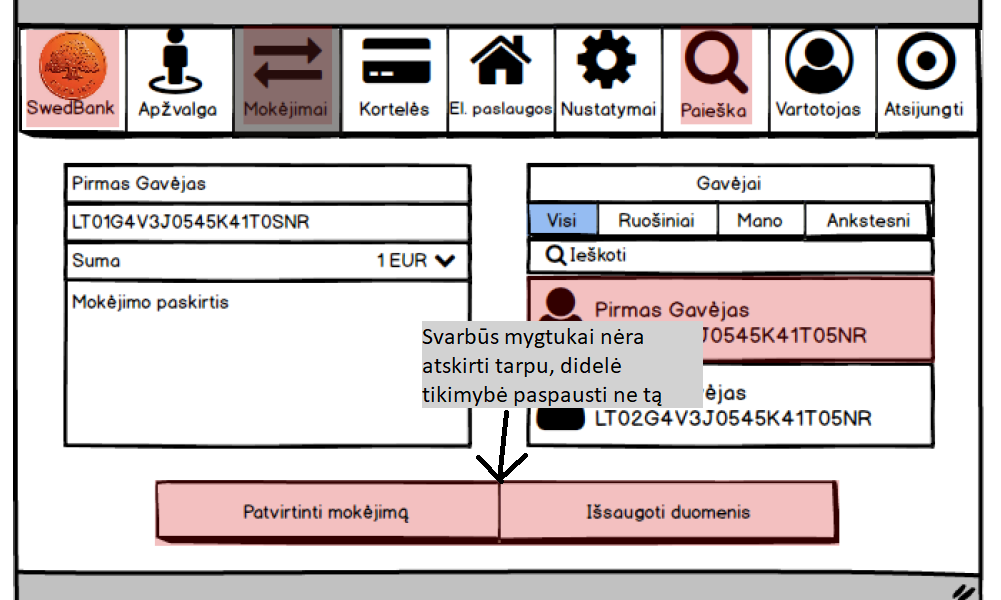
\includegraphics[scale=0.55]{MokejimoPatvirtinimasKlaiduPrevencija.png}
  \caption{Mygtukų išdėstymas vietinių mokėjimų lange}
	\label{fig:klaiduPrevencijaMygtukai}
\end{figure}
\hyperref[lentele:klaiduPrevencijaJ]{Defektas} yra didelės reikšmės, kadangi mokėjimo pavedimas yra rimta operacija, todėl klaidingas jos įvygdymas sukeltų reikšmingų nepatogumų sistemos naudotojui. Šią problemą galima spręsti keliais būdais: 1) mygtukus reiktų atitraukti į priešingas puses, kad tarp jų būtų tarpas užtikrinantis didesnį paspaudimų tikslumą. 2) prieš patvirtinant mokėjimą galima parodyti papildomą langą, kuriame vartotojas galėtų patvirtinti, kad nori atlikti šią operaciją.

\subsection{Pažintinė peržvalga}

\begin{center}
\begin{longtable}[!htb]{|p{5cm}|p{5cm}|p{5cm}|}
	\caption{Justo Tvarijono vertinimas}
\endfirsthead
\endhead
	\hline
	Užduoties žingsniai & Ar aiškiai matoma, ką daryti? & Ar suprantamas atsakas? \\ \hline
	1. Atsidaryti mokėjimų langą & Taip, meniu juostoje mygtukas pavadinimu "Mokėjimai" vartotojui siejasi su jo siekiamu tikslu & Taip, vartotojas gali matyti ar padarė teisingą žingsnį, kadangi šis paspaudimas priartino jį prie tikslo (vartotojas gavo konkretesnius mokėjimo pasirinkimus) \\ \hline
	2. Pasirinkti vietiniu mokėjimus & Taip, tarp lange išdėstytų mygtukų nesunku rasti ieškomą(su pavadinimu "vietiniai mokėjimai") & Nevisiškai, vartotojas, kuris dažniau naudojasi sistema supras, kad yra tame lange, kuriame turi būti, tačiau jame niekur neparašyta, kad tai vietinių mokėjimų langas, tai gali suklaidinti kai kuriuos vartotojus. \\ \hline
	3. Suvesti duomenis & Taip, įvedimo laukai gerai matomi, ant kiekvieno laukelio parašyta, ką jame reikia įvesti(tačiau ant jo paspaudus paaiškinimai digsta) & Ne, sistema niekaip neparodo ar įvesti duomenys yra tinkami. Būtų galima pavaizduoti žalią varnelę prie įvedimo lauko, jeigu duomenys yra validūs. \\ \hline
	4. Patvirtinti mokėjimą & Taip, ekrano apačioje yra mygtukas, kurio tekstas pakankamai aiškiai nurodo, kad jis skirtas mokėjimo patvirtinimui & Taip, patvirtinus mokėjimą išoką patvirtinimo langas, iš kurio vartotojas sužino, kad jo mokėjimas sėkmingai įgyvendintas. \\ \hline
\end{longtable}
\end{center}
\subsection{Apibendrinimas}
\section{Justo Tvarijono maketo vertinimas}
\subsection{Euristinis tikrinimas}
\subsection{Pažintinė peržvalga}
\subsection{Apibendrinimas}
\section{Michal Stankevič maketo vertinimas}
\subsection{Euristinis tikrinimas}
\subsection{Pažintinė peržvalga}
\subsection{Apibendrinimas}
\section{Išvados}
\section{Priedai}
	\begin{itemize}
		\item Justas Tvarijonas - VU MIF programų sistemų sistemos 3 kurso studentas.
		\item Džiugas Mažulis - VU MIF programų sistemų sistemos 3 kurso studentas.
		\item Michal Stankevič - VU MIF programų sistemų sistemos 3 kurso studentas.
	\end{itemize}
\end{document}
